\section*{Notizen, Skizzen und andere kreative Ideen}
\label{pg:rätsel_lösungen}
\newcommand{\fibelnotesimg}{%
	\begin{tikzpicture}[remember picture, overlay]
		\node[anchor=north east, yshift=-0.5cm] at (current page text area.north east)
		{
\includegraphics[width=5cm]{res/tango_accessories-text-editor.pdf}};
	\end{tikzpicture}%
}
\fibelnotesimg

\begin{tikzpicture}[remember picture, overlay]
	\node[anchor=west, xshift=1.2cm, yshift=-3mm, inner sep=0] at (current page.west)
	{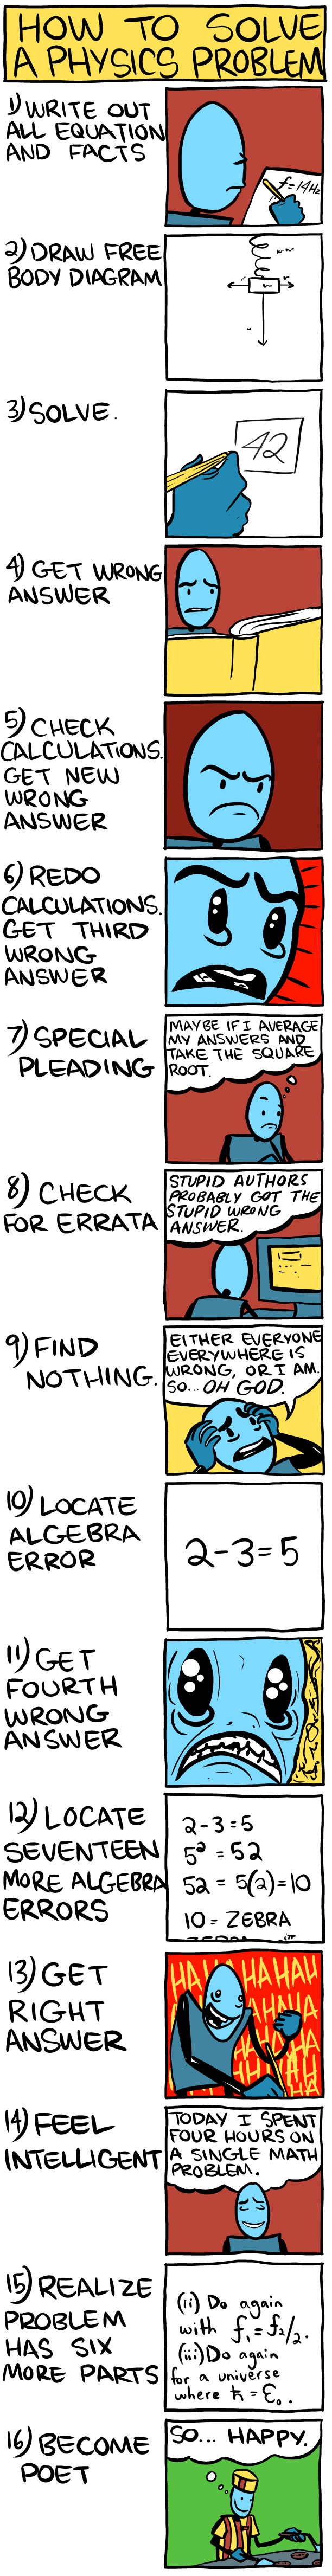
\includegraphics[width=0.18\textwidth, height=0.95\textheight]{res/smbc/2013-06-16.png}};
\end{tikzpicture}

\vspace{\fill}
\hfill
\rotatebox{180}{
	\begin{minipage}{0.8\textwidth}
		Lösungen zum Sprichwörterrätsel:\\
		Scherben bringen Glück;
		Ein voller Bauch studiert nicht gern;
		Steter Tropfen höhlt den Stein;
		Wo Licht ist, ist auch Schatten;
		Wer anderen eine Grube gräbt, fällt selbst hinein
		
		\medskip
		
		Lösungen zum Münsterrätsel:\\
		\ref{itm:rätsel_bieranstalt}b,
		\ref{itm:rätsel_ethanol}b,
		\ref{itm:rätsel_götter}a (nach den Göttern Thingsus [Kriegsgott], Freya [Liebesgöttin] und Donar [Wettergott]),
		\ref{itm:rätsel_xi}a,
		\ref{itm:rätsel_pyramide}a,
		\ref{itm:rätsel_bruce}c,
		\ref{itm:rätsel_burger}a und d ;-),
		\ref{itm:rätsel_chemiker}~selbsterklärend,
		\ref{itm:rätsel_elefanten}c
	\end{minipage}
}

% Fügt automatisch Notizseiten ein, sodass die Seitenzahl ein Vielfaches
% von 4 ist
\colorlet{currentcolor}{.}
\notespages[
	multiple=4,
	endpages=4,
	titletext={},
	notesstyle=text,
	notestextalign=none,
	% aktuelle Textfarbe verwenden, da \notespages standardmäßig {gray}{0.7}
	% als Farbe auf Notizseiten setzt
	notestext=\color{currentcolor}\fibelnotesimg
]
